\bigskip

\bigskip

\begin{multicols}{2}
\textbf{Ingredients}
\begin{itemize}
\item 1 smoked sausage (Hillshire farms $\sim$14 oz) \newline (1,190 kCal/ 49 gP/ 105 gF/ 21 gC)
\item 2 lbs peeled \& deveined shrimp \newline(900 kCal/ 218 gP/ 2gF/ 2 gC)
\item 1 yellow onion \quad (45 kCal/ 1 gP/ 0 gF/ 11 gC)
\item Celery ($\sim$8 ribs) \quad (45 kCal/ 2 gP/ 0 gF/ 11 gC)
\item $\sim 5$ cloves of garlic (minced) (65 kCal /3 gP/ 0 gF/ 15 gC)
\item 1 bell pepper \quad (18 kCal/ 1 gP/ 0 gF/ 4 gC)
\item 4 cups long grain white rice \quad (2560 kCal/ 48 gP/ 0 gF/ 576 gC)
\item 3 small cans tomato paste \quad (525 kCal/ 15 gP/ 0 gF/ 105 gC)
\item 1 28 oz can diced tomatoes \quad (175 kCal/ 7 gP/ 0 gF/ 35 gC)
\item 2 boxes (64 oz) chicken stock \quad (80 kCal/ 8 gP/ 0 gF/ 8gC)
\item 2 tbsp olive oil \quad (238 kCal/ 0 gP/ 28 gF/ 0 gC)
\item 2-3 tbsp. creole seasoning
\item 2 bay leaves 
\item salt to taste





\end{itemize}


\columnbreak
\textbf{Procedure:}
\medskip


\begin{enumerate}
\item In a large pan, cook shrimp in olive oil until pink. Remove from pan and set aside. Sautee garlic, onions, and celery in pan in another tablespoon of olive oil until onions are translucent. Add tomato paste and stir frequently over medium heat until tomato paste darkens, being careful not to burn the tomato paste.


\medskip
\item Add about 2 cups of chicken stock to pan to deglaze, making sure to scrape off any browned bits from the bottom of the pan and stir until smooth. At this point, the mixture should be pretty thick. 
\medskip

\item Add seasoning and diced tomatoes. Cook over medium-low heat for 10 minutes and add the sausage and shrimp. Cook for another 10 minutes. Add the rest of the chicken stock and check the seasoning, stirring thoroughly. 
\newline 

 \item Add rice, and cook until rice has absorbed the liquid and is cooked through (20-25 minutes). Be sure not to let rice burn on the bottom of the pan. Stir frequently and remove from heat when it has reached the right consistency. 
\end{enumerate}

\begin{table}[H]
  \begin{center}
    \caption{Macro totals}
    \label{tab:table1}
    \begin{tabular}{c|c|c|c} % <-- Alignments: 1st column left, 2nd middle and 3rd right, with vertical lines in between
      \textbf{Calories} & \textbf{Protein} & \textbf{Fat} & \textbf{Carbs}\\
      \hline
      5,841 kCal & 352 g & 138 g & 788 g\\
    \end{tabular}
  \end{center}
\end{table}
\end{multicols}


%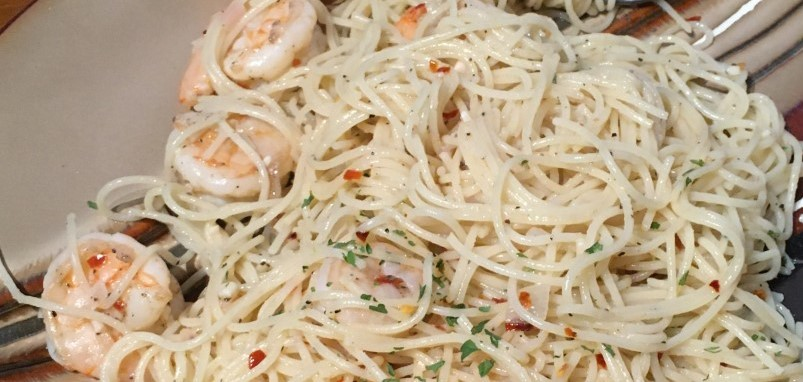
\includegraphics[scale=0.35]{Pasta/Shrimp Scampi/Shrimp Scampi.jpg}
%\end{center}